\documentclass{standalone}

\usepackage{tikz}
\usetikzlibrary{arrows}
\usetikzlibrary{decorations.markings}
\usetikzlibrary{calc}

\begin{document}

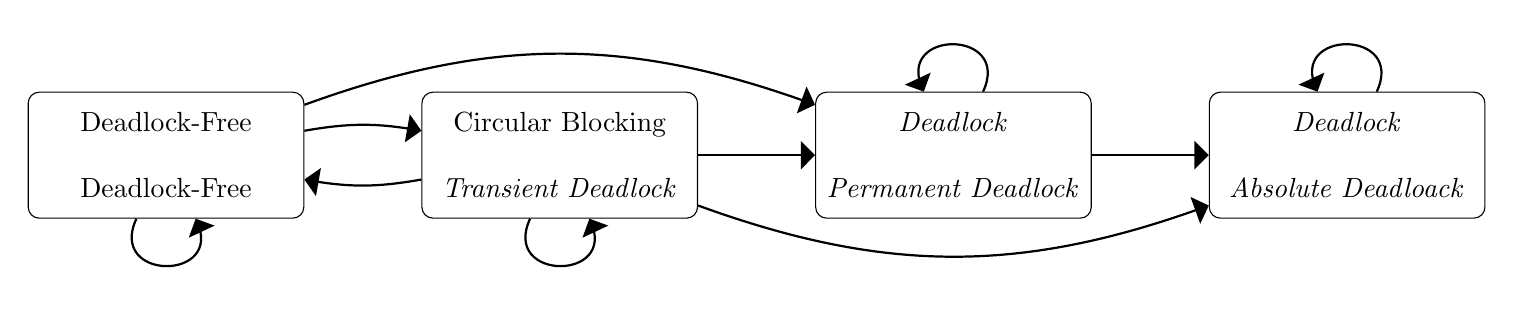
\begin{tikzpicture}

\node[align=center, draw=black, minimum height = 1.6cm, minimum width = 3.5cm, rounded corners] (deadlockfree) at (0, 0) {Deadlock-Free\\ \Vhrulefill \\Deadlock-Free};
\node[align=center, draw=black, minimum height = 1.6cm, minimum width = 3.5cm, rounded corners] (circularblocking) at (5, 0) {Circular Blocking\\ \Vhrulefill \\\textit{Transient Deadlock}};
\node[align=center, draw=black, minimum height = 1.6cm, minimum width = 3.5cm, rounded corners] (deadlock) at (10, 0) {\textit{Deadlock}\\ \Vhrulefill \\\textit{Permanent Deadlock}};
\node[align=center, draw=black, minimum height = 1.6cm, minimum width = 3.5cm, rounded corners] (absolutedeadlock) at (15, 0) {\textit{Deadlock}\\ \Vhrulefill \\\textit{Absolute Deadloack}};

\draw[thick, black, -triangle 90] (deadlockfree) [out=10, in=170, looseness=1] to (circularblocking);
\draw[thick, black, -triangle 90] (circularblocking) [out=-170, in=-10, looseness=1] to (deadlockfree);
\draw[thick, black, -triangle 90] (circularblocking) to (deadlock);
\draw[thick, black, -triangle 90] (deadlock) to (absolutedeadlock);
\draw[thick, black, -triangle 90] (deadlockfree) [out=20, in=160, looseness=1] to (deadlock);
\draw[thick, black, -triangle 90] (circularblocking) [out=-20, in=-160, looseness=1] to (absolutedeadlock);

\draw[thick, black, -triangle 90] (deadlockfree) [out=-115, in=-65, looseness=3] to (deadlockfree);
\draw[thick, black, -triangle 90] (circularblocking) [out=-115, in=-65, looseness=3] to (circularblocking);
\draw[thick, black, -triangle 90] (deadlock) [out=65, in=115, looseness=3] to (deadlock);
\draw[thick, black, -triangle 90] (absolutedeadlock) [out=65, in=115, looseness=3] to (absolutedeadlock);


\end{tikzpicture}

\end{document}
